\section{Тэхнічныя рашэнні для рэалізацыі праектаванай IP-сеткі}

\subsection{Выбар пратакола маршрутызацыі}

У якасці пратаколу маршрутызацыі можа быць абраны RIP, OSPF або якой-небудзь іншай пратакол маршрутызацыі, напрыклад IS-IS або EIGRP, у залежнасці ад тапалогіі і задач сеткі. RIP адносіцца да пратаколаў маршрутызацыі тыпу «вектар-адлегласць», тады як IS-IS і OSPF ставяцца да пратаколаў стану звяна. EIGRP з'яўляецца гібрыдным пратаколам. Разгледзім гэтыя пратаколы маршрутызацыі больш падрабязна.

\subsubsection{Пратакол OSPF.}
OSPF --- гэта адкрыты пратакол маршрутызацыі, які базіруецца на алгарытме пошуку найкарацейшага шляху (Open Shortest Path First --- OSPF). OSPF мае дзве асноўныя характарыстыкі: пратакол з'яўляецца адкрытым, г. зн. яго спецыфікацыя з'яўляецца грамадскім здабыткам, ён грунтуецца на алгарытме SPF. Алгарытм SPF часам называюць алгарытмам Дейкстры па імені яго аўтара. OSPF з'яўляецца іерархічным пратаколам маршрутызацыі з аб'яўленнем стану аб канале злучэння (link-state). Ён быў спраектаваны як пратакол работы ўнутры сеткавай вобласці --- AS (Autonomous System), якая ўяўляе сабой групу маршрутызатараў і сетак, аб'яднаных па іерархічным прынцыпе і якія знаходзяцца пад адзіным кіраваннем і сумесна выкарыстоўваюць агульную стратэгію маршрутызацыі. У якасці транспартнага пратаколу для маршрутызацыі ўнутры AS OSPF выкарыстоўвае IP-пратакол. Абмен інфармацыяй аб маршрутах ўнутры AS пратакол OSPF ажыццяўляе праз абмен паведамленнямі аб станах канала злучэнняў паміж маршрутызатарамі і сеткамі вобласці (link-state advertisement - LSA). Гэтыя паведамленні перадаюцца паміж аб'ектамі сеткі, якія знаходзяцца ў межах адной і той жа іерархічнай вобласці --- гэта можа быць як уся AS, так і некаторая група сетак ўнутры дадзенай AS. У LSA-паведамленні пратаколу OSPF ўключаецца інфармацыя аб падлучаных інтэрфейсах, пра параметры маршрутаў і іншых зменных. Па меры назапашвання маршрутызатарамі OSPF інфармацыі аб стане маршрутаў вобласці, яны разлічваюць найкарацейшы шлях да кожнага вузла, выкарыстоўваючы алгарытм SPF. Пры гэтымразлік аптымальнага маршруту ажыццяўляецца дынамічна ў адпаведнасці са зменамі тапалогіі сеткі.

Для розных тыпаў IP-сeрвісу (відаў паслуг вышэйшага ўзроўню, якія вызначаюцца значэннем поля TOS IP-пакета), OSPF можа разлічваць свае аптымальныя маршруты на падставе параметраў, найбольш крытычных для дадзенага тыпу сeрвісу. Напрыклад, якая-небудзь прыкладная праграма можа ўключыць патрабаванне аб тым, што пэўная інфармацыя з'яўляецца тэрміновай. Калі OSPF мае ў сваім распараджэнні каналы з высокім прыярытэтам, то яны могуць быць выкарыстаны для транспарціроўкі тэрміновых дэйтаграм.

OSPF падтрымлівае механізм, які дазваляе працаваць з некалькімі раўнапраўнымі маршрутамі паміж двума аб'ектамі сеткі. Гэта дазваляе істотна паменшыць час перадачы дадзеных і больш эфектыўна выкарыстоўваць каналы сувязі.

Акрамя таго, OSPF-пратакол падтрымлівае аўтэнтыфікацыю змяненняў маршрутаў. Гэта азначае, што толькі тыя маршрутызатары, якія маюць пэўныя правы, могуць ажыццяўляць маршрутызацыю пакетаў. Гэта дазваляе, пры адпаведнай настройкі правоў сістэмы маршрутызатараў, перадаваць па сетцы канфідэнцыйныя паведамленні, ведаючы загадзя, што яны праходзяць толькі па пэўных маршрутах.

Да таго ж, так як OSPF гэта пратакол стану канала, а не пратакол вектара адлегласцяў, ён мае і іншыя характарыстыкі, якія робяць яго лепш ў адносінах да RIP:
\begin{enumerate}
    \item OSPF можа разлічыць асобны набор маршрутызатараў для кожнага тыпу сeрвісу IP (type-of-service). Гэта азначае, што для любога пункта прызначэння можа быць некалькі пунктаў у табліцы маршрутызацыі, па адным для кожнага тыпу сeрвісу IP;
    \item Кожнаму інтэрфейсу прызначаецца кошт. Ён можа быць прызначаны на падставе прапускной здольнасці, часу вяртання, надзейнасці або па якому-небудзь іншаму параметру. Асобны кошт можа быць прызначаны для кожнага тыпу сeрвісу IP.
    \item Калі існуе некалькі маршрутаў да аднаго пункта прызначэння з аднолькавым коштам, OSPF размяркоўвае трафік аднольнакава паміж гэтымі маршрутамі. Гэта называецца балансіроўкай нагрузкі.
    \item Каналы пункт-пункт паміж маршрутызатарамі не маюць IP адрасоў на кожным канцы. Гэта называецца сеткамі без адраса (unnumbered). Такі падыход дазваляе зэканоміць IP адрасы.
\end{enumerate}

\subsubsection{Пратакол RIP.}
Пры выкарыстанні пратакола RIP кожны маршрутызатар рэгулярна (а таксама па асабліваму запыце па-за раскладам) рассылае сваім суседзям абвесткі, якія змяшчаюць адлегласць (вымеранае ў ліку крокаў маршрутызацыі) да ўсіх вядомых яму сетак. Сусед павялічвае адлегласць на адзін (калі казаць дакладней, то на метрыку інтэрфейсу), уносіць гэтыя маршруты ў сваю табліцу і рассылае іх усім сваім суседзям (у тым ліку і папярэдняга, але той ігнаруе іх, таму што ўжо ведае маршруты ад сябе). Максімальная даўжыня маршруту ў RIP складае 15 крокаў маршрутызацыі (hops).

Калі нейкая сетка становіцца недаступнай, то маршрутызатары працягваюць перасылаць адзін аднаму маршруты, кожны раз павялічваючы метрыку. У рэшце рэшт метрыка дасягае велічыні 16, якая азначае ў тэрмінах RIP бясконцасць, або недаступную сетку.

RIP --- самы просты з пратаколаў дынамічнай маршрутызацыі, але ён мае істотныя недахопы: марудную збежнасць, абмежаваны памер сеткі, вялікі аб'ём службовага трафіку (кожны раз рассылаецца маршрутная табліца цалкам). Апошняе робіць выкарыстанне RIP вельмі дарагім, напрыклад, у сотавых сетках. Тым не менш, RIP дагэтуль можа быць актуальны ў адносна простых і малых сетках.

\subsubsection{Пратакол IS-IS.}
IS-IS і OSPF з'яўляюцца пратаколамі стану каналаў (link state protocols), і абодва пратаколы выкарыстоўваюць алгарытм Дэйкстры для знаходжання найкарацейшага шляху. Таксама абодва пратаколы падтрымліваюць сеткавыя маскі рознай даўжыні, могуць прымяняць мультыкаставую рассылку для знаходжання найбліжэйшых маршрутызатараў, выкарыстоўваючы hello пакеты, і могуць падтрымліваць аўтэнтыфікацыю пры абнаўленні маршрутаў.

У той час як OSPF першапачаткова пабудаваны для маршрутызацыі IP адрасоў і сам працуе як пратакол 3 ўзроўню на IP, IS-IS першапачаткова з'яўляецца сеткавым узроўнем мадэлі OSI. Шырокае ўкараненне IP адрасоў спрыяла росту папулярнасці OSPF. IS-IS не выкарыстоўвае IP адрасы ў якасці маршрутаў. Ён з'яўляецца нейтральным ў дачыненні да сеткавых адрасоў, у той час OSPF быў спраектаваны для IPv4. Гэта дазваляе з лёгкасцю выкарыстоўваць IS-IS для IPv6. Для падтрымкі IPv6 сетак OSPF быў перапісаны ў OSPFv3.

Маршрутызатары IS-IS будуюць тапалагічнаe ўяўленне сеткі. Гэтая мапа паказвае падсеткі, якія IS-IS маршрутызатар можа дасягнуць, і шлях з самым нізкім коштам (найлепшы), які выкарыстоўваецца для перанакіравання трафіку.

Асноўнае адрозненне OSPF і IS-IS заключаецца ў тым як яны дзеляць аўтаномную сістэму на зоны і як ажыццяўляецца маршрутызацыя паміж зонамі. Недахоп IS-IS у тым, што маршрутызатары 2-га ўзроўню могуць мець зносіны толькі з такімі ж маршрутызатарамі, у 1-га ўзроўню --- такая ж сітуацыя. Для ўзаемадзеяння паміж маршрутызатарамі 1-га і 2-га ўзроўню і адпаведнымі зонамі выкарыстоўваюцца маршрутызатары ўзроўню 1-2. У OSPF зоны адмяжоўвацца інтэрфейсамі на маршрутызатары, такім чынам памежны маршрутызатар (area border router, ABR) можа знаходзіцца ў некалькіх зонах адначасова, эфектыўна ствараючы межы ўнутры сябе. Тады як межы IS-IS зон знаходзяцца паміж маршрутызатарамі ўзроўню 2 або ўзроўню 1-2, што робіць маршрутызатар IS-IS часткай толькі адной зоны. Таксама IS-IS не падтрымлівае нулявую зону (магістральную вобласць, праз якую можа прайсці ўвесь міжабласны трафік). Лагічным тлумачэннем гэтага з'яўляецца тое, што OSPF стварае сетку з тапалогіяй зорка з многімі зонамі перасякальнымі з нулявой, тады як IS-IS стварае лагічную тапалогію з асноўным узроўнем з маршрутызатараў 2 ўзроўню, філіялаў --- маршрутызатараў ўзроўню 1-2 і асобных абласцей з маршрутызатараў ўзроўню 1.

У пратаколе OSPF больш пашырэнняў і дадатковых функцый. Аднак пратакол IS-IS адпраўляе меншую колькасць службовага трафіку і можа маштабавацца для вялікіх сетак.

\subsubsection{Пратакол EIGRP.}
EIGRP --- удасканалены дыстанцыйна-вектарны пратакол дынамічнай маршрутызацыі, распрацаваны кампаніяй Cisco.

Дадзены пратакол маршрутызацыі папулярны ў лакальных сетках па некалькіх прычынах: настройка EIGRP даволі простая, ён устойлівы, хутка канвергуецца і для яго характэрна невысокая верагоднасць узнікнення колцавых маршрутаў. Для гэтага пратакола не трэба старанна планаваць сетку, ён просты ў канфігурацыі і пры гэтым добра маштабуецца і можа выкарыстоўвацца ў буйных сетках.Галоўны недахоп EIGRP --- закрыты стандарт. І хоць у дадзены момант кампанія Cisco адкрыла гэты пратакол, абсталяванне іншых вытворцаў можа не падтрымліваць дадзены пратакол маршрутызацыі.

Для нашай праектуемай сеткі будзем выкарыстоўваць пратакол OSPF у сувязі
з тым, што ён мае выдатныя характарыстыкі ў параўнанні з іншымі, што ён
адкрыты пратакол, а значыць пашыраецца выбар сеткавага абсталявання.
Неабходна адзначыць, што дадзены пратакол валодае высокай гібкасцю, ўлічвае асаблівасці сеткі і пры фарміраванні табліц маршрутызацыі ўлічвае прапускную здольнасць ліній, што дазваляе гібка настрайваць табліцу маршрутызацыі і тым самым паскорыць маршрутызацыю трафіку.

На малюнку \ref{figure: OSPF Header} прадстаўлены загаловак OSPF пакета.

\begin{figure}[h!]
    \centering
    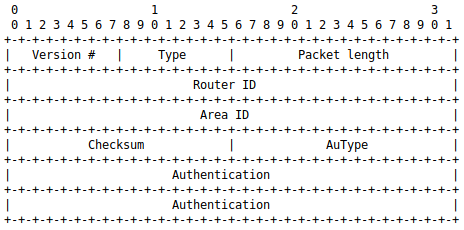
\includegraphics{ospf_header.png}
    \vspace{-0.7\baselineskip}
    \caption{Загаловак OSPF пакета}
    \label{figure: OSPF Header}
\end{figure}

Разгледзім структуру загалоўка OSPF пакета:
\begin{enumerate}
    \item Version --- версія OSPF пратакола;
    \item Type --- тып OSPF пакета:
    \begin{enumerate}
        \item Hello;
        \item Database Description;
        \item Link State Request;
        \item Link State Update;
        \item Link State Acknowledgment;
    \end{enumerate}
    \item Packet length --- даўжыня пакета ў байтах;
          уключае ў сябе стандартны OSPF загаловак;
    \item Router ID --- ідэнтыфікатара маршрутызатара крыніцы пакета;
    \item Area ID --- 32-бітны ідэнтыфікатар вобласці, да якой належыць пакет;
    \item Checksum --- кантрольная сума для праверкі змесціва пакета на памылкі;
    \item AuType --- тып аўтэнтыфікацыі:
    \begin{enumerate}
        \item 0 --- без аўтэнтыфікацыі;
        \item 1 --- пароль, які перадаецца адкрытым тэкстам;
        \item 2 --- MD5 аўтэнтыфікацыя;
    \end{enumerate}
    \item Authentication --- 64-бітнае полe для паведамлення аўтэнтыфікацыі.
\end{enumerate}

\subsection{Абаненцкі доступ да праектуемай сеткі}

\subsection{Выбар сеткавага абсталявання}
